\documentclass{standalone}
\usepackage{tikz}
\usetikzlibrary{arrows.meta, positioning, shapes.geometric}

\begin{document}
	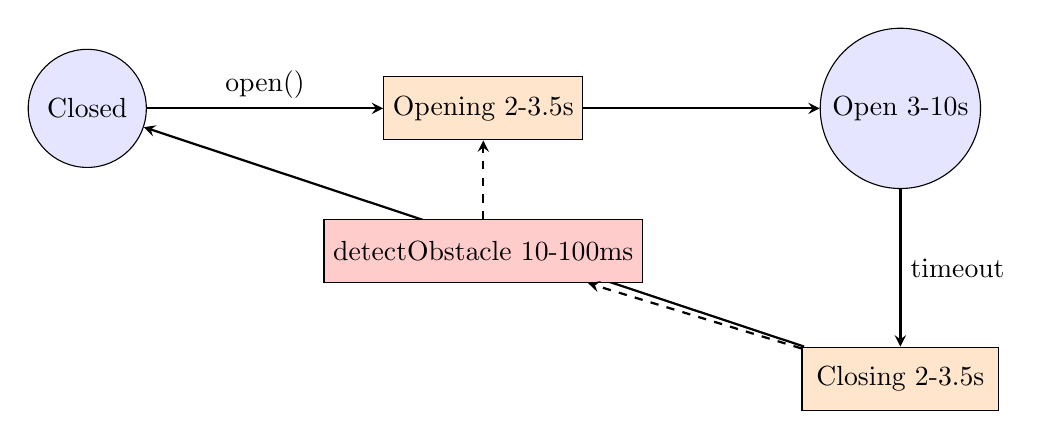
\begin{tikzpicture}[
		state/.style={circle, draw, fill=blue!10, minimum size=1.5cm},
		action/.style={rectangle, draw, fill=orange!20, minimum width=2.5cm, minimum height=0.8cm},
		arrow/.style={->, >=stealth, thick}
		]
		\node[state] (closed) {Closed};
		\node[action, right=3cm of closed] (opening) {Opening 2-3.5s};
		\node[state, right=3cm of opening] (open) {Open 3-10s};
		\node[action, below=2cm of open] (closing) {Closing 2-3.5s};
		
		\draw[arrow] (closed) -- (opening) node[midway, above] {open()};
		\draw[arrow] (opening) -- (open);
		\draw[arrow] (open) -- (closing) node[midway, right] {timeout};
		\draw[arrow] (closing) -- (closed);
		
		\node[action, below=1cm of opening, fill=red!20] (detect) {detectObstacle 10-100ms};
		\draw[arrow, dashed] (closing) -- (detect);
		\draw[arrow, dashed] (detect) -- (opening);
	\end{tikzpicture}
\end{document}